\textbf{Autor: Andreas, Torben, Marvin}

In der Modulsicht wird der Aufbau der in der konzeptionellen Sicht dargestellten Komponenten beschrieben. Die Modulsicht wird in die Pakete Common, Model, Business Logic, View, Exception, Util und Controller unterteilt und wird durch UML-Diagramme dargestellt.

Eingaben auf der Website werden vom Paket View auf den Controller weitergeleitet. Das Paket Controller kann Anfragen auf das Model weiterleiten. Das Paket Model kümmert sich darum, die vom Controller angefragten Daten aus der Datenbank zu laden und diese wieder zurück an den Controller zu leiten. Dabei können Anfragen versendet werden, die z.B. einer mathematischen Funktionalität benötigt. Dafür greift der Controller auf das Paket Businesslogic zu, auf dem sämtliche mathematische Berechnung durchgeführt, Passwörter, Nachrichten, etc. encrypted und decrypted oder Kriterien für die Operationen ausgewertet werden.

Im Folgenden stellen wir die UML-Klassendiagramme der einzelnen Module dar. Die Beschreibung einzelner Klassen, Attribute und Methoden ist den JavaDoc-Kommentaren in dem mitgegebenen Maven-Projekt zu entnehmen.


%%%%%%%%%%%%%%%
% Businesslogic
%%%%%%%%%%%%%%%

\newpage
\subsection{Businesslogic}

Das Paket Businesslogic enthält die Klassen, die Aufgaben der Geschäftslogik übernehmen.

\begin{figure}[H]
	\centering
  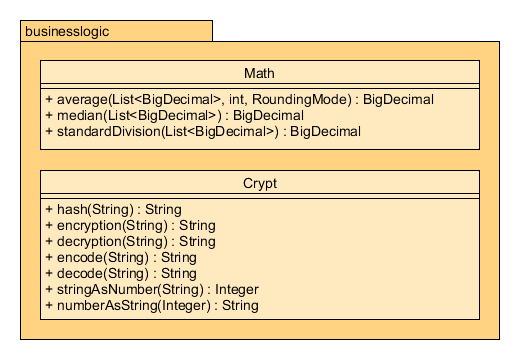
\includegraphics[width=\textwidth,height=10cm,keepaspectratio]{../UMLDiagramme/businesslogic/gfx/4_package_businesslogic.png}
	\caption{Package businesslogic}
\end{figure}

%%%%%%%%%%%%%%%
% Common
%%%%%%%%%%%%%%%

\newpage
\subsection{Common}

Das Paket Common fasst die Pakete \texttt{exception}, \texttt{model} und \texttt{util} zusammen. Das folgende Paketdiagramm verdeutlicht den Zusammenhang genauer.

\begin{figure}[H]
	\centering
  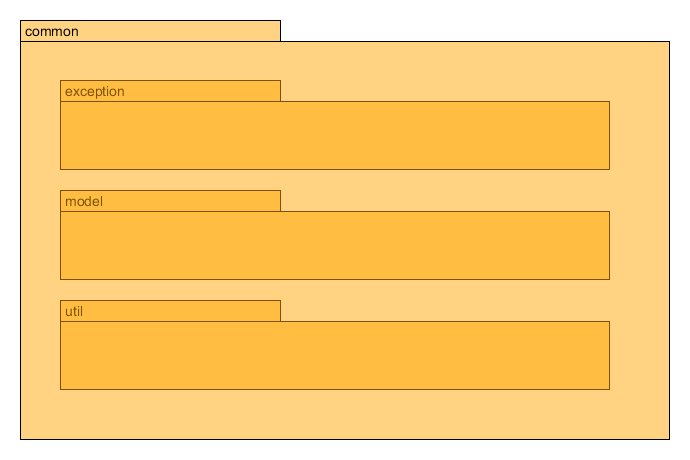
\includegraphics[width=\textwidth,height=10cm,keepaspectratio]{../UMLDiagramme/common/gfx/4_package_common.png}
	\caption{Package common}
\end{figure}

%%%%%%%%%%%%%%%
% Exception
%%%%%%%%%%%%%%%

\newpage
\subsubsection{Exception}

Dieses Paket enthält alle programmspezifischen Exceptions.

\begin{figure}[H]
	\centering
  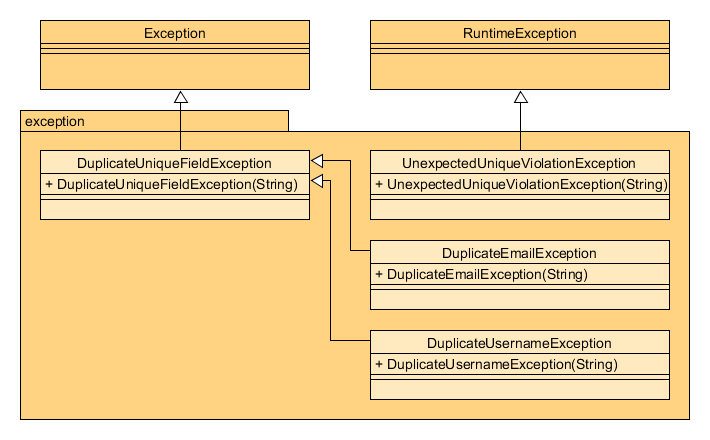
\includegraphics[width=\textwidth,height=10cm,keepaspectratio]{../UMLDiagramme/common/exception/gfx/4_package_exception.png}
	\caption{Package common.exception}
\end{figure}

%%%%%%%%%%%%%%%
% Model
%%%%%%%%%%%%%%%

\newpage
\subsubsection{Model}

Das Paket \texttt{Model} enthält alle Datenklassen der Applikation.

Aufgrund der Übersichtlichkeit wurden die einzelnen Klassen des Pakets in seperate Diagramme unterteilt. Da die Klasse \texttt{JPAEntity} in jedem der folgenden Diagramme auftaucht, wird der Inhalt der Klasse lediglich im ersten Diagramm (siehe \ref{a}) aufgeführt. Die Attribute und Methoden von \texttt{JPAEntity} werden in den anderen Klassendiagrammen leer gelassen, um Übersichtlichkeit zu bewahren.

\begin{figure}[H] \label{a}
	\centering
  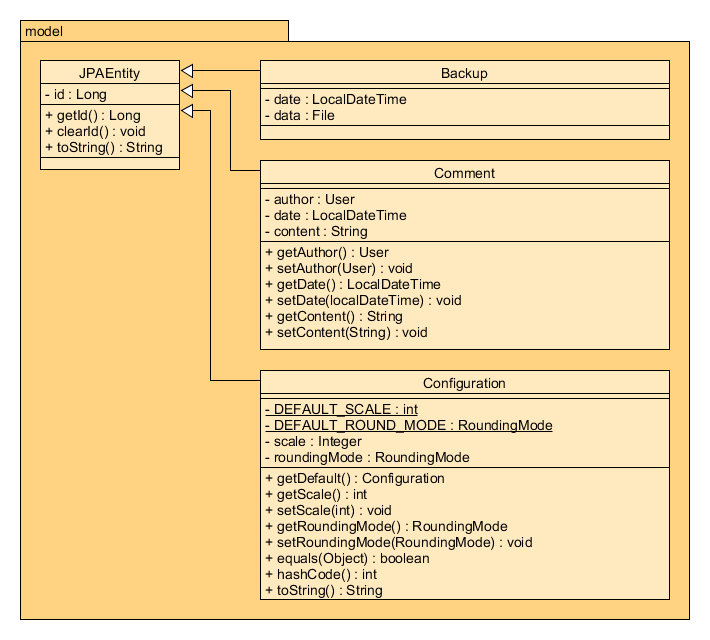
\includegraphics[width=\textwidth]{../UMLDiagramme/common/model/gfx/4_package_model_part_1.png}
	\caption{Package common.model}
\end{figure}

\begin{figure}[H]
	\centering
  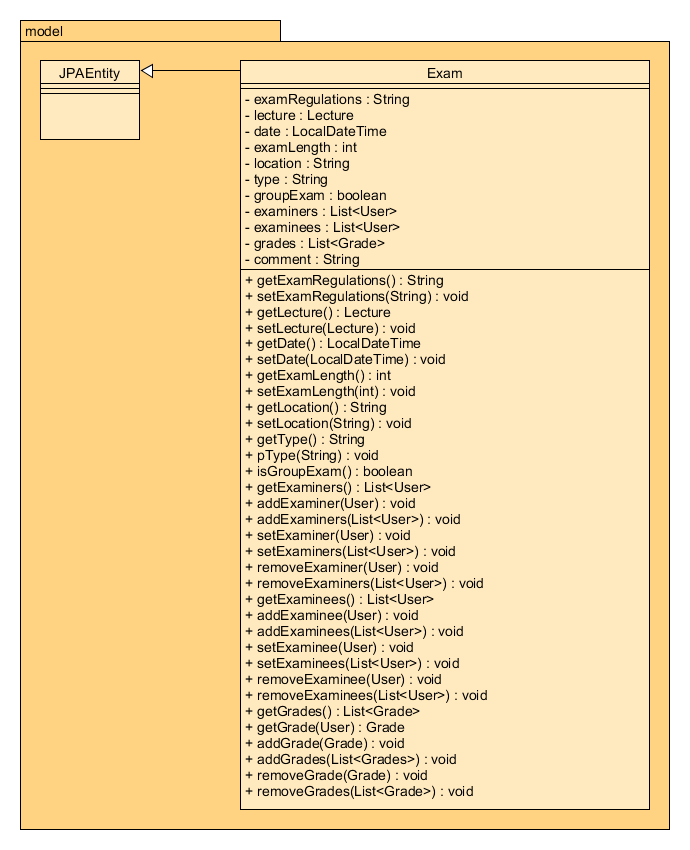
\includegraphics[width=\textwidth]{../UMLDiagramme/common/model/gfx/4_package_model_part_2.png}
	\caption{Package common.model}
\end{figure}

\begin{figure}[H]
	\centering
  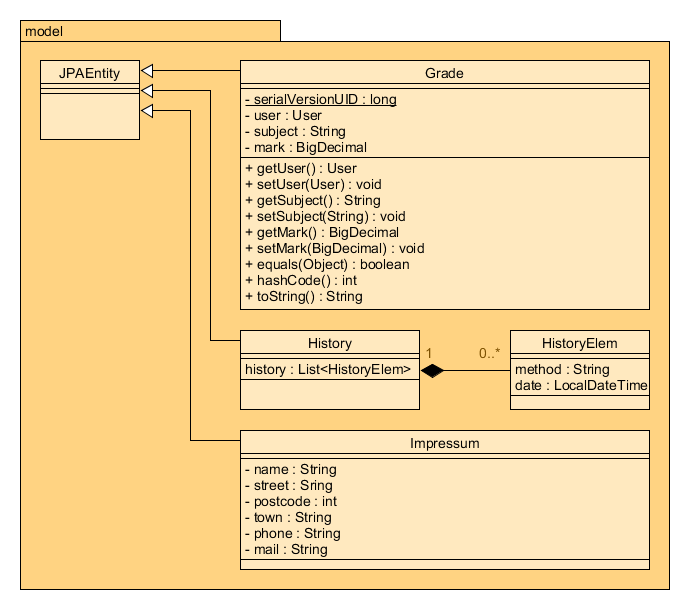
\includegraphics[width=\textwidth]{../UMLDiagramme/common/model/gfx/4_package_model_part_3.png}
	\caption{Package common.model}
\end{figure}

\begin{figure}[H]
	\centering
  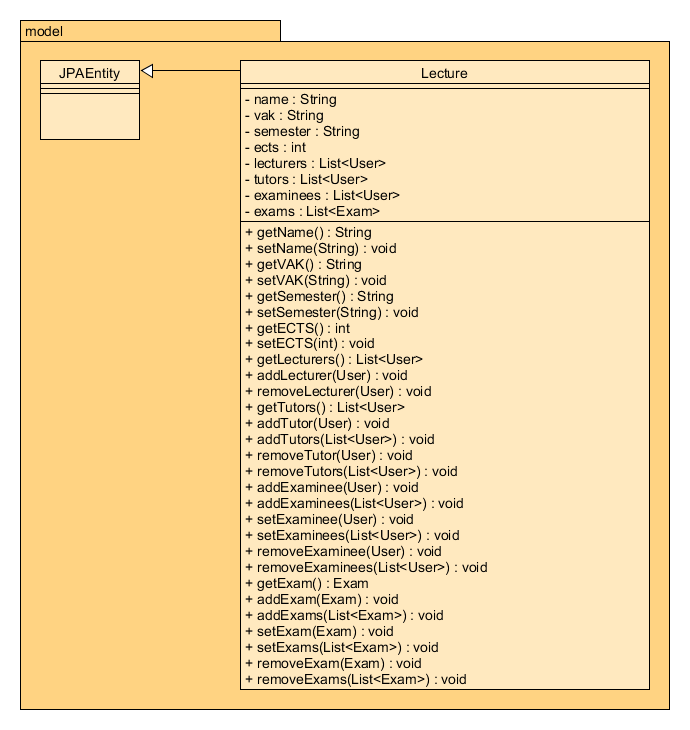
\includegraphics[width=\textwidth]{../UMLDiagramme/common/model/gfx/4_package_model_part_4.png}
	\caption{Package common.model}
\end{figure}

\begin{figure}[H]
	\centering
  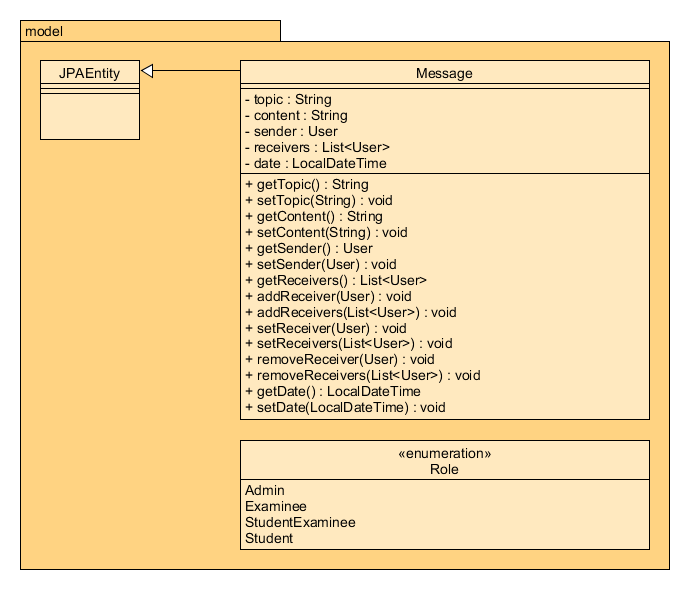
\includegraphics[width=\textwidth]{../UMLDiagramme/common/model/gfx/4_package_model_part_5.png}
	\caption{Package common.model}
\end{figure}

\begin{figure}[H]
	\centering
  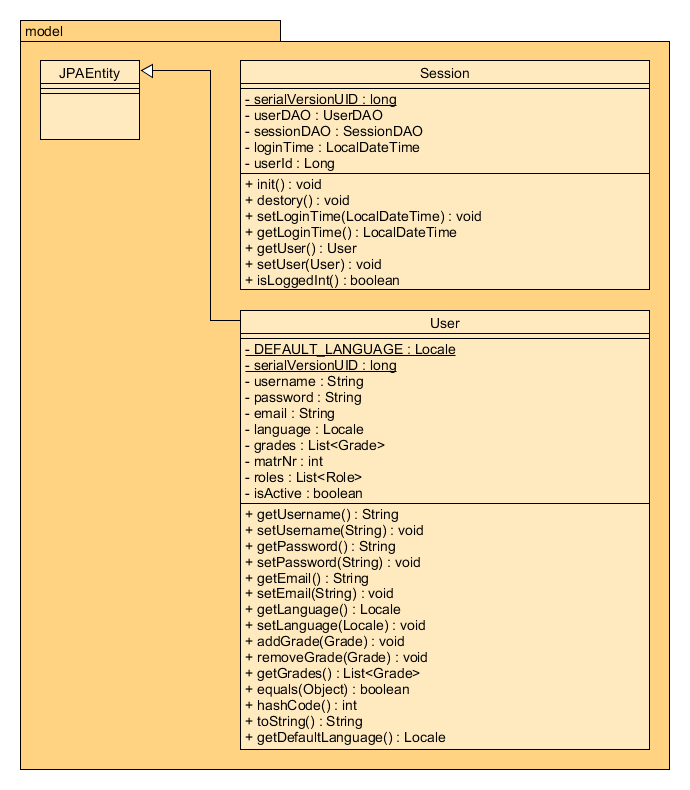
\includegraphics[width=\textwidth]{../UMLDiagramme/common/model/gfx/4_package_model_part_6.png}
	\caption{Package common.model}
\end{figure}

%%%%%%%%%%%%%%%
% Util
%%%%%%%%%%%%%%%

\newpage
\subsubsection{Util}

Das \texttt{Util}-Paket enthält unterstützende Funktionen für die Applikation.

\begin{figure}[H]
	\centering
  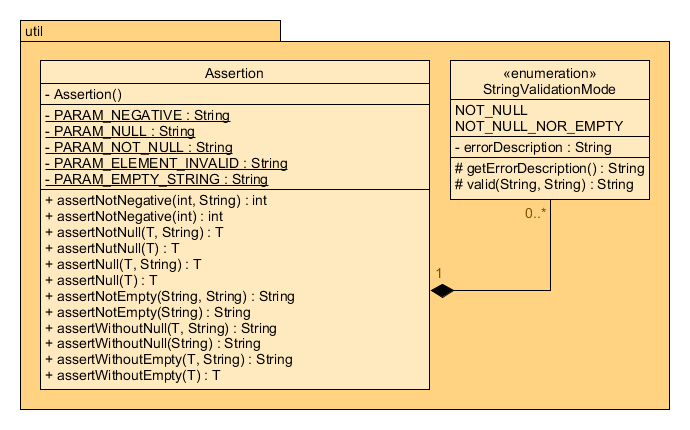
\includegraphics[width=\textwidth]{../UMLDiagramme/common/util/gfx/4_package_util.png}
	\caption{Package common.util}
\end{figure}

%%%%%%%%%%%%%%%
% Controller
%%%%%%%%%%%%%%%

\newpage
\subsection{Controller}

Enthält Backing Beans, die die Controller der Facelets realisieren.

Aufgrund der Übersichtlichkeit wurden die Klassen des Controllers in verschiedene Klassendiagramme unterteilt. Die in der Abbildung \ref{s} bis zur Abbildung \ref{e} dargestellten Klassen befinden sich alle innerhalb des Pakets Controller. Außerdem wurde die AbstractBean, die in jedem der entsprechenden Klassendiagramme vorkommt in der Abbildung \ref{s} genauer dargestellt und im Folgenden ohne Konstruktor und Methoden gezeigt, um die Darstellungen möglichst übersichtlich zu halten.

\begin{figure}[H] 
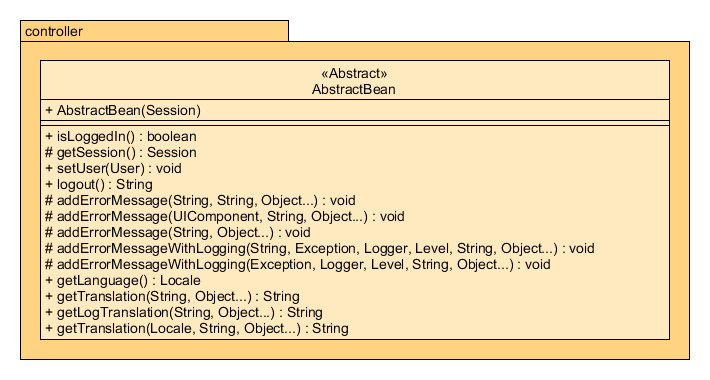
\includegraphics[width=\textwidth]{../UMLDiagramme/controller/gfx/4_package_controller_part_0.png}
	\caption{Package controller}
	\label{s}
\end{figure}

\begin{figure}[H] \label{cal}
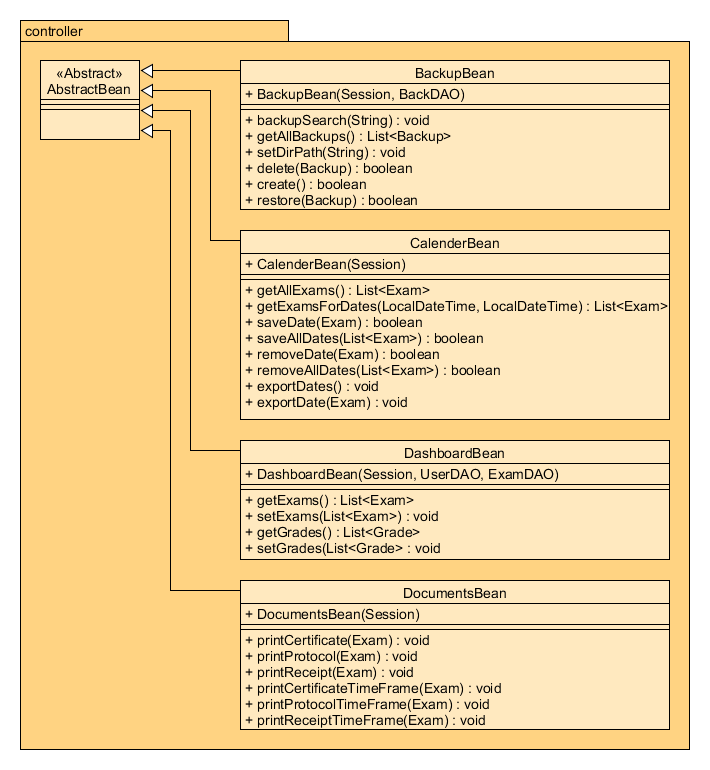
\includegraphics[width=\textwidth]{../UMLDiagramme/controller/gfx/4_package_controller_part_1.png}
	\caption{Package controller}
\end{figure}

\begin{figure}[H]
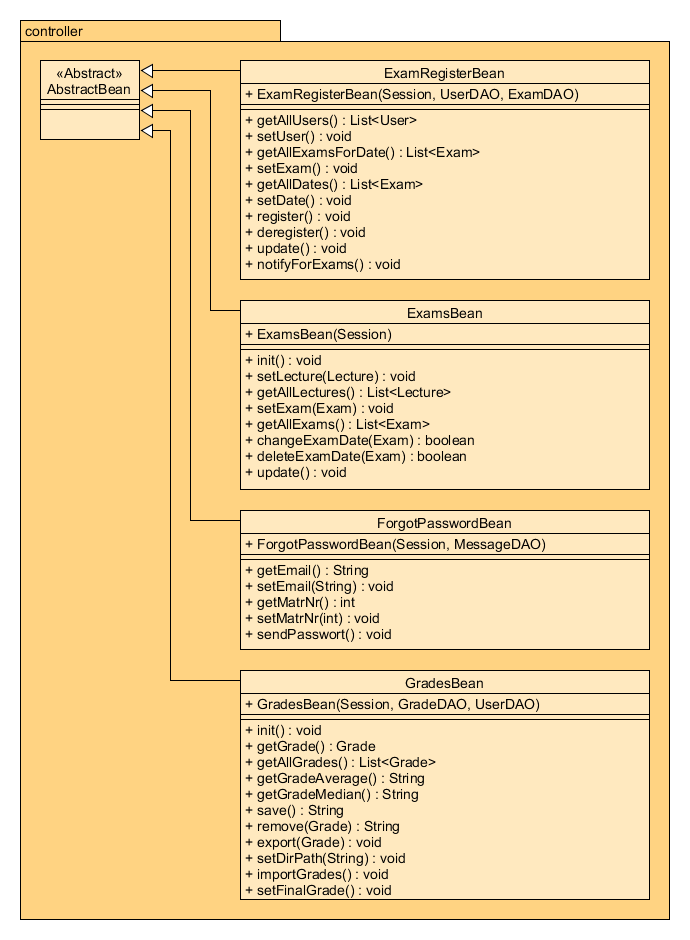
\includegraphics[width=\textwidth]{../UMLDiagramme/controller/gfx/4_package_controller_part_2.png}
	\caption{Package controller}
\end{figure}

\begin{figure}[H]
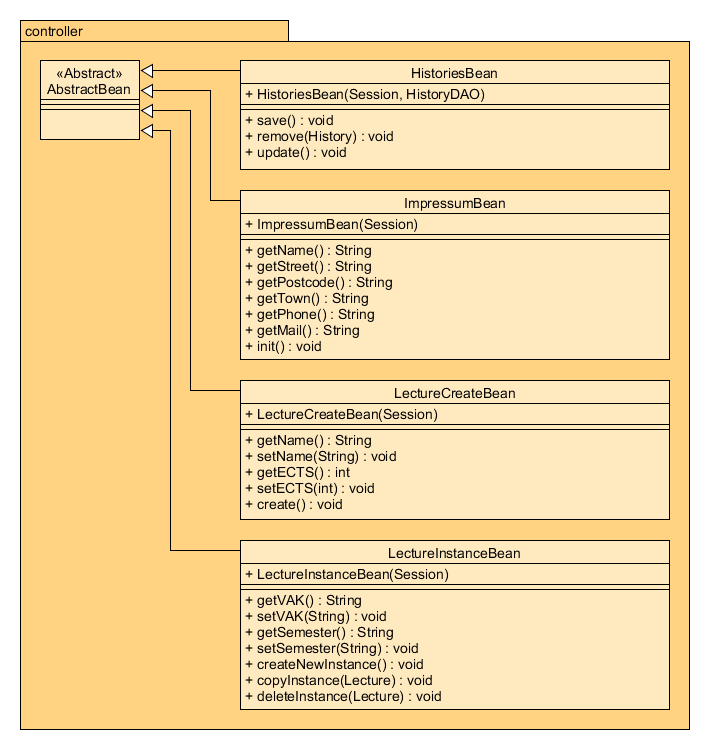
\includegraphics[width=\textwidth]{../UMLDiagramme/controller/gfx/4_package_controller_part_3.png}
	\caption{Package controller}
\end{figure}

\begin{figure}[H]
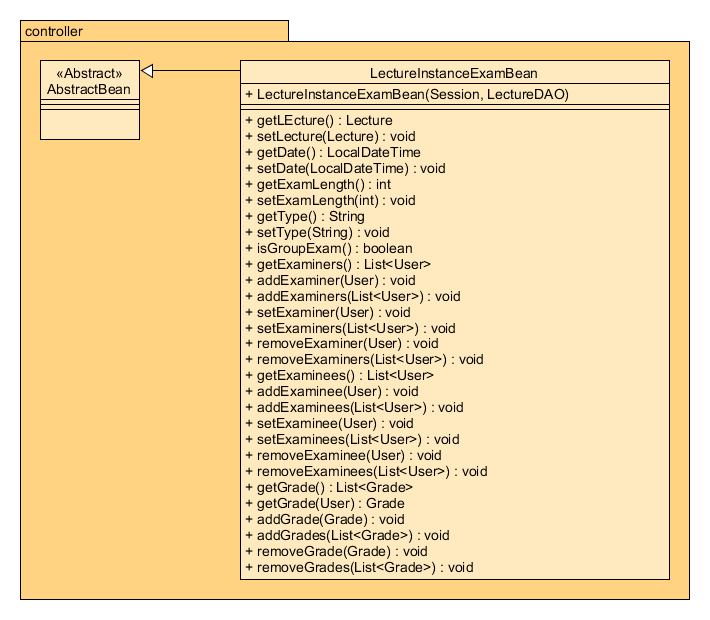
\includegraphics[width=\textwidth]{../UMLDiagramme/controller/gfx/4_package_controller_part_4.png}
	\caption{Package controller}
\end{figure}

\begin{figure}[H]
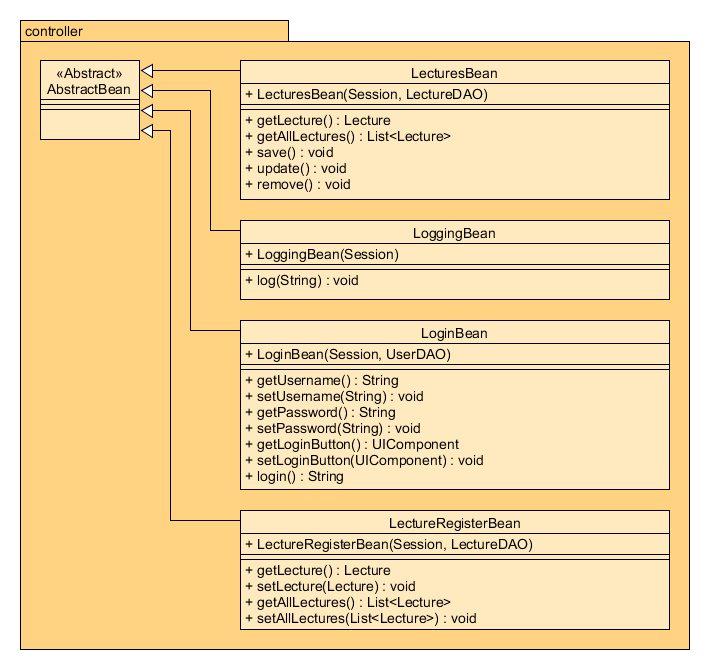
\includegraphics[width=\textwidth]{../UMLDiagramme/controller/gfx/4_package_controller_part_5.png}
	\caption{Package controller}
\end{figure}

\begin{figure}[H]
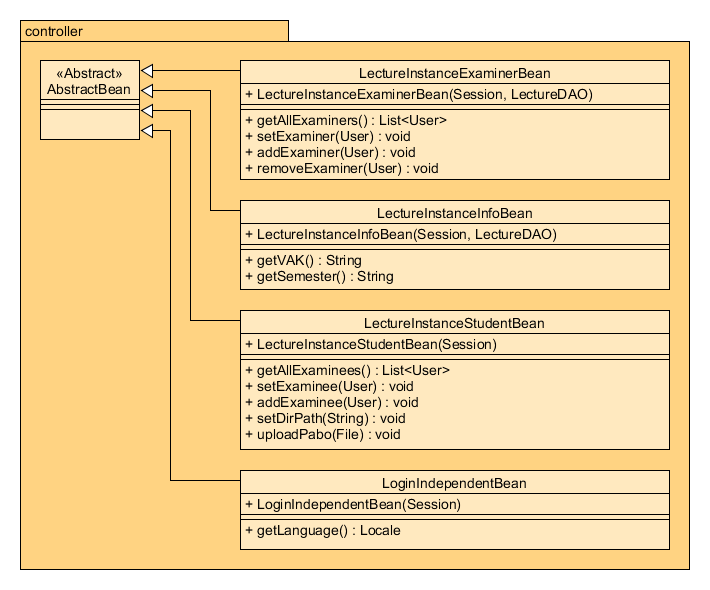
\includegraphics[width=\textwidth]{../UMLDiagramme/controller/gfx/4_package_controller_part_6.png}
	\caption{Package controller}
\end{figure}

\begin{figure}[H] 
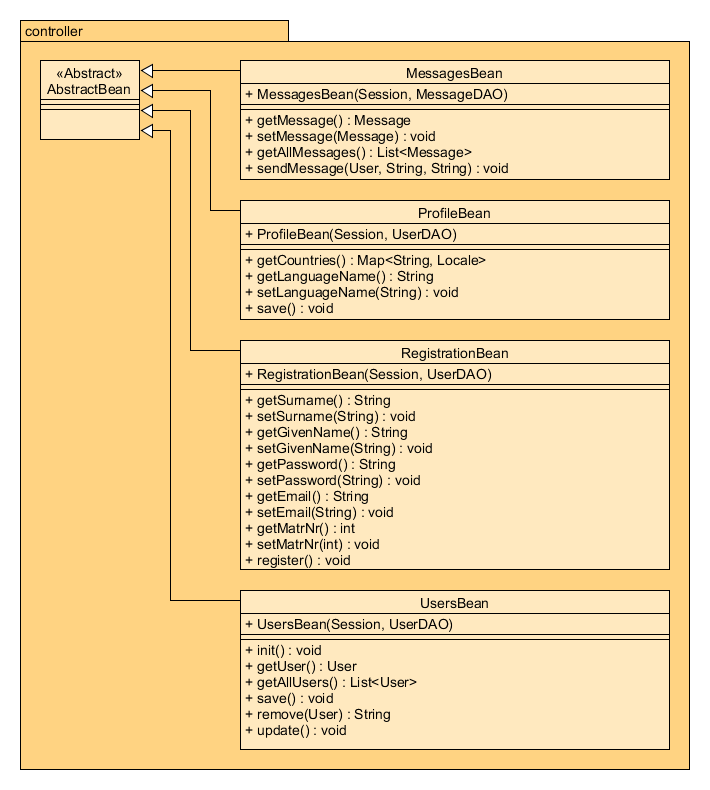
\includegraphics[width=\textwidth]{../UMLDiagramme/controller/gfx/4_package_controller_part_7.png}
	\caption{Package controller}
	\label{e}
\end{figure}

%%%%%%%%%%%%%%%
% Persistence
%%%%%%%%%%%%%%%


\subsection{Persistence}
\texttt{Persistence} enthält Klassen, die Aufgaben im Hinblick auf das Persistieren der Daten der Applikation übernehmen. Klassen dieses Pakets interagieren mit der Datenbank.}

\begin{figure}[H] \label{per}
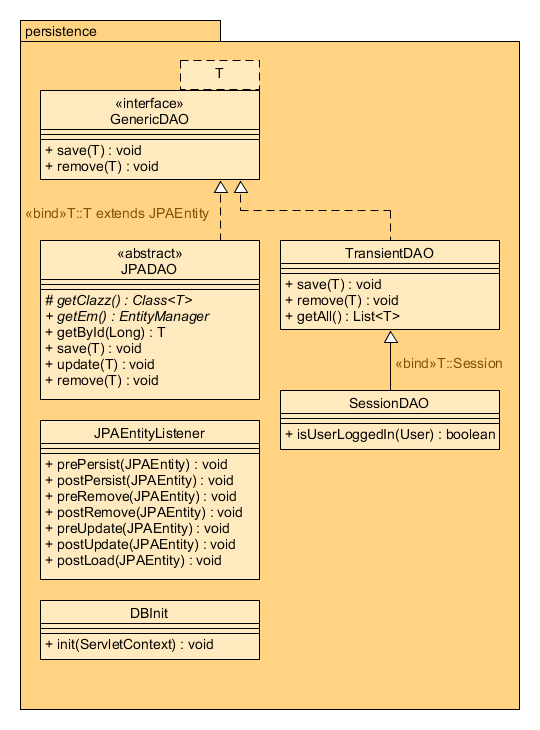
\includegraphics[width=\textwidth]{../UMLDiagramme/persistence/gfx/4_package_persistence_part_0.png}
	\caption{Package persistence}
\end{figure}

\begin{figure}[H]
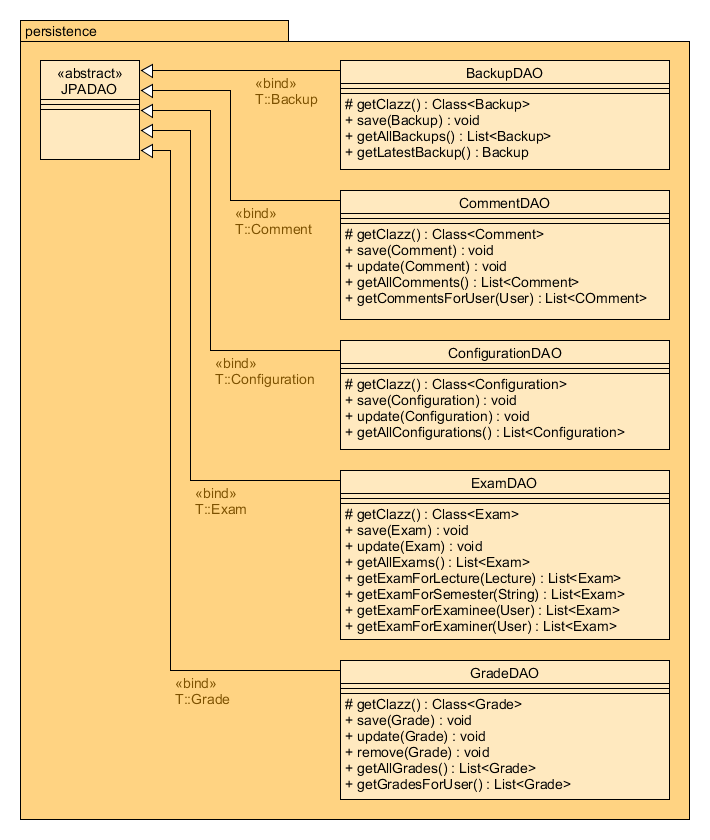
\includegraphics[width=\textwidth]{../UMLDiagramme/persistence/gfx/4_package_persistence_part_1.png}
	\caption{Package persistence}
\end{figure}

\begin{figure}[H]
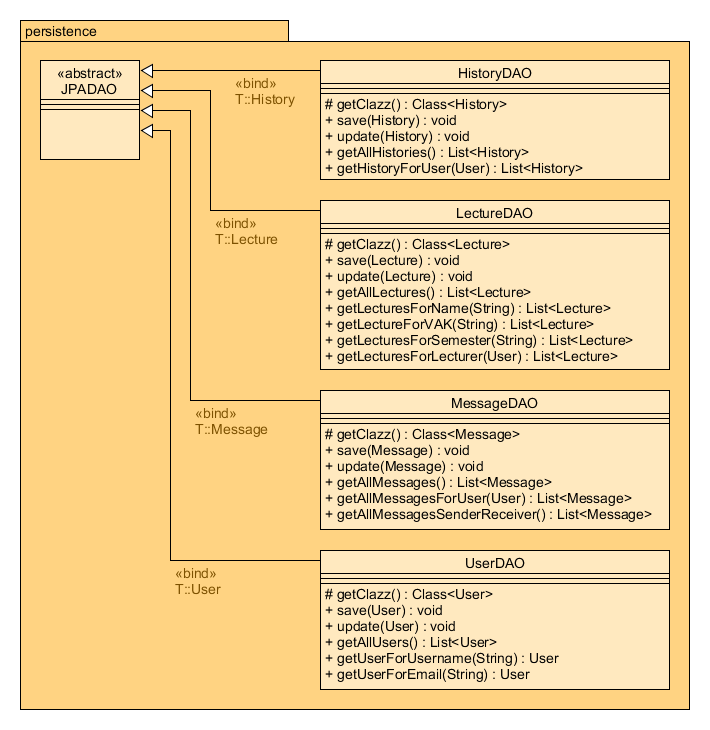
\includegraphics[width=\textwidth]{../UMLDiagramme/persistence/gfx/4_package_persistence_part_2.png}
	\caption{Package persistence}
\end{figure}

%%%%%%%%%%%%%%%
% View
%%%%%%%%%%%%%%%

\newpage
\subsection{View}

Die \texttt{View} enthält alle \texttt{xhtml}-Seiten der Applikation. Die Startseite ist hierbei die in der Grafik grün markierte \texttt{index.xhtml}. Das folgende Diagramm stellt die in der Applikation enthaltenen Seiten dar.

\begin{figure}[H]
	\centering
  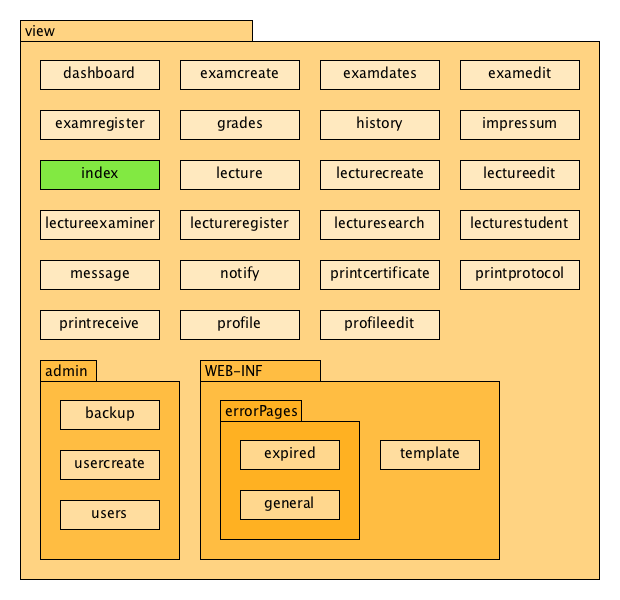
\includegraphics[width=\textwidth]{../UMLDiagramme/view/gfx/4_package_view.png}
	\caption{Package view}
	\label{fig 2}
\end{figure}


\subsection{Anwendung der Strategien auf die Modulsicht}
Alle vorher getroffenen Entscheidungen  und Strategien (\ref{K5}) aus der konzeptionellen Sicht wurden übernommen und weiterentwickelt. Die vorher getroffene Modularisierung wurde konkretisiert durch das Hinzufügen der benötigten Klassen und Methoden.\\

\textbf{S8: Historisierung der Nutzeraktionen:}\\
Die Nutzung von Log4j wird in dem Modul HistoriesBean (Paket: Controller) und LoggingBean (Paket: Controller) erfolgen. Die Methoden zum Loggen der Nutzeraktionen werden dort implementiert, wobei LoggingBean zum Debuggen der Anwendung genutzt wird. HistoriesBean wird relevante Aktionen des Nutzers historiseren und visualisieren.\\

\textbf{S10: Benutzung auf mobilen Geräten:}\\
Alle XHTML-Seiten in dem Paket View werden auf das responsive Design setzen.  Dazu werden von den Seiten CSS-Dateien eingebunden, die das Design für unterschiedliche Auflösungen definieren.\\

\textbf{S12: Das Anbinden der Datenbank - JPA:}\\
Die Datenbank wird in dem Paket Persistence mithilfe von JPA angesteuert. \\

\textbf{S13: Das Anbinden der Datenbank - Zugriffe:}\\
Die Argumente eines Methodenaufrufs werden durch die Klasse Assertion (Paket Util) geprüft. Dadurch sollen fehlerhafte oder bösartige Zugriffe unterbunden werden.\\

\textbf{S15: Mehrsprachigkeit:}\\
Alle XHTML-Seiten in dem Paket View erhalten rendern je nach Sprachauswahl den deutschen oder englischen Text einer Seite. Beide Sprachversionen werden für die textuellen Inhalte im XHTML-Code hinterlegt.\\

\textbf{S17: Benachrichtigung der Nutzer:}\\
Die Benachrichtigungen haben eine Datenstruktur in der Klasse Message (Paket Model). Das Verschicken und Empfangen läuft unter Zuhilfenahme von JMail in der Klasse MessageBean (Paket Controller).\\ 

\textbf{S19: Nutzerverwaltung - Konto:}\\
Jeder Nutzer hat ein eigenes Konto. Die Datenstruktur für den Nutzer ist in der Klasse User (Paket Model) angegeben. Die Daten des Benutzers werden in der Klasse UserDAO (Paket Persistence) persistiert. Jeder Nutzer ist eindeutig identifizierbar über die E-Mail.
Jeder Nutzer hat eine eigene Session und in der Klasse <enumeration> Role (Paket Model) sind die Nutzergruppen definiert. Jede Komponente von View fragt die Nutzergruppe des Benutzers ab und rendert nur relevante Bestandteile.\\ 

\textbf{S20: Nutzerverwaltung - ACID:}\\
Die Zugriffe auf die Datenbank erfolgt über JPA, dadurch sind ACID-Eigenschaften gewährleistet.\\

\textbf{S21: Nutzerverwaltung - Session:}\\
Jeder Nutzer erhält eine eigene Session.  Die Datenstruktur der Session ist in der Klasse Session (Paket: Model). Außerdem wird in jeder Komponente von View ein Scope für die Interaktionen angegeben.\\

\textbf{S22: Nutzerverwaltung - Verschlüsselung:}\\
Die Klasse Crypt (Paket BusinessLogic) bietet Verschlüsselung- und Entschlüsselungmethoden für andere Pakete, wie z.B. Controller oder Model, an. Dadurch können die Daten sicher übertragen und gespeichert werden.  \\

\textbf{S24: Daten-Backup erzeugen:}\\
Die Erzeugung und Verwaltung des Daten-Backups wird in der Klasse  BackupDAO (Paket Persistence) geregelt. Die passende Datenstruktur wird in der Klasse Backup (Paket Model) erzeugt. Die View rendert die Seite backup.xhtml nur für Benutzer mit der Rolle Admin.\\

\textbf{S27: Aktualisierung der Inhalte:}\\
Es wird keine Nebenläufigkeit im Softwaresystem verwendet. Die Zugriffe auf die Datenbank erfolgen hintereinander. Generell gilt First-Come-First-Serve bei der Vergabe von gemeinsamen Resourcen, wie z.B. Prüfungstermine.